\documentclass{article}
\usepackage{a4wide}
\usepackage[english]{babel}
\usepackage{amsmath}
\usepackage{amssymb}
\usepackage{dsfont}
%\usepackage[dvips]{epsfig}
%\usepackage{graphicx}
\usepackage{fancyhdr}
\usepackage{listings}
\usepackage{nomencl}
\usepackage[pdftex]{graphicx}

\pagestyle{fancy}
\lhead{\footnotesize \parbox{11cm}{A.J. H\"ormer, E. Vontobel, A. Novacek}}
\rhead{\footnotesize {Plexos Project}}
\chead{\footnotesize {TET4135}}

\title{Report Plexos Project}
\author{Andreas Johann H\"ormer, Eva Vontobel, Adam Novacek}
\date{\today}

\begin{document}
\thispagestyle{empty}
\maketitle
\thispagestyle{empty}
%\\[5cm]
\begin{center}
TET4135 Energiplanlegging\\[3cm]
Lab group:
\begin{itemize}
\item Andreas Johann H\"ormer
\item Eva Vontobel
\item Adam Novacek\\[3cm]
\end{itemize}
Report delivered: \\[6cm]
FACULTY OF INFORMATION TECHNOLOGY, MATHEMATICS AND ELECTRICAL ENGINEERING\\
NORWEGIAN UNIVERSITY OF SCIENCE AND TECHNOLOGY
\end{center}
\thispagestyle{empty}
\newpage
\tableofcontents
\thispagestyle{empty}
\newpage
\section*{Abstract}
\thispagestyle{empty}

\newpage
\setcounter{page}{1}
\section{Introduction}

\section{Theory}
\subsection{Methods in present work}
\subsection{intermittent resource handling}
\subsection{reservoir hydro handling}
\subsection{region exchange}
\subsubsection{Advantages}
\subsubsection{Disadvantages}
\subsection{investment initiatives for renewable sources}
\begin{itemize}
\item investment support\\
One time financial support to cover part of the investment costs.  The support is large enough to make the investment profitable. Some differences can be used for fine tuning, e.g. more support for wind power in areas with less wind.
\begin{itemize}
\item advantages
\begin{itemize}
\item possibility of finetuning
\end{itemize}
\item disadvantages
\begin{itemize}
\item requires much capital at beginning
\item no incentive to roduce
\item limited security for investor
\item in case of fine tuning: much administration
\end{itemize}
\end{itemize}
\item tendering\\
Auction for a certain amount of capacity which shall be installed. Won by the offers requiring the lowest support. This initiative is also done as investment support, but with a tendering procedure. Providers are asked for support bids, the cheapest one gets the support.
\begin{itemize}
\item advantages
\begin{itemize}
\item competition between suppliers, therefore lower costs than investment support
\end{itemize}
\item disadvantages
\begin{itemize}
\item same as investment support, but
\item less predictability
\item prone to corruption
\end{itemize}
\end{itemize}
\item feed-in tariff\\
A fixed price for feeded kWh is payed for a predefined period.
\begin{itemize}
\item advantages
\begin{itemize}
\item promotion of mid-term and long-term technologies
\item investment security for producer
\end{itemize}
\item disadvantages
\begin{itemize}
\item possible risk of technology overfunding
\end{itemize}
\end{itemize}
\item premium\\
Like feed-in tariff, but instead of a fixed price an additional amount per kWh is paid to the producer.
\begin{itemize}
\item advantages
\begin{itemize}
\item market based
\end{itemize}
\item disadvantages
\begin{itemize}
\item less certainty than feed-in tariff
\end{itemize}
\end{itemize}
\item green certificates
This is a nordic system for supporting renewables. Some amount of certified energy has to be bought from energy suppliers, otherwise they are penalized. The intention is to build as much renewables as possible in short time. From 2020 new renewables are not certified any more, so the possibility to get enough certified power decreases and the risk of getting penalized increases.
\begin{itemize}
\item advantages
\begin{itemize}
\item control of total amount of renewables
\item efficient market-based solution
\end{itemize}
\item disadvantages
\begin{itemize}
\item less certainty than feed-in
\item complex
\item high administration costs
\end{itemize}
\end{itemize}
\end{itemize}

\section{Analysis}
\subsection{MT Schedule}
The medium term schedule is done for one year. Three different scenarios (low, normal, high inflow) to the reservoirs in Norway and Sweden are simulated. The different scenarios are described below.
\subsubsection{normal inflow scenario}
For this case a normal inflow scenario was chosen. The inflow accords to the average inflow in a year in Norway and Sweden.
\paragraph{optimal generation dispatch\\}
The optimal generation dispatch for normal inflow for Germany can be seen in figure \ref{fig:MTgenerationGnormal}. The generation dispatch for swedish generation units can be seen in figure \ref{fig:MTgenerationSnormal}, the norwegian dispatch is shown in figure \ref{fig:MTgenerationNnormal}.
\begin{figure}[htbp]
\begin{center}
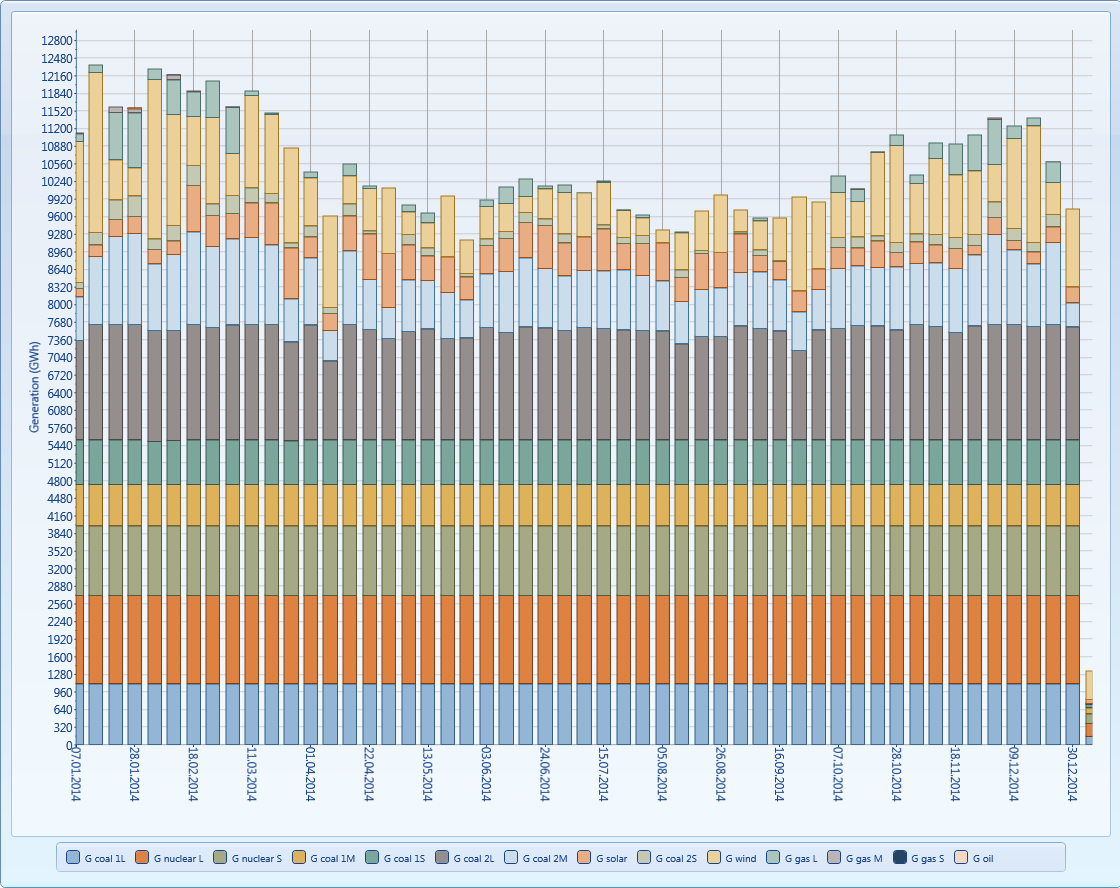
\includegraphics[width=14cm,keepaspectratio=true]{figures/MTgenerationG}
\caption{Optimal generation dispatch for Germany 2014 with normal inflow}
\label{fig:MTgenerationGnormal}
\end{center}
\end{figure}
\begin{figure}[htbp]
\begin{center}
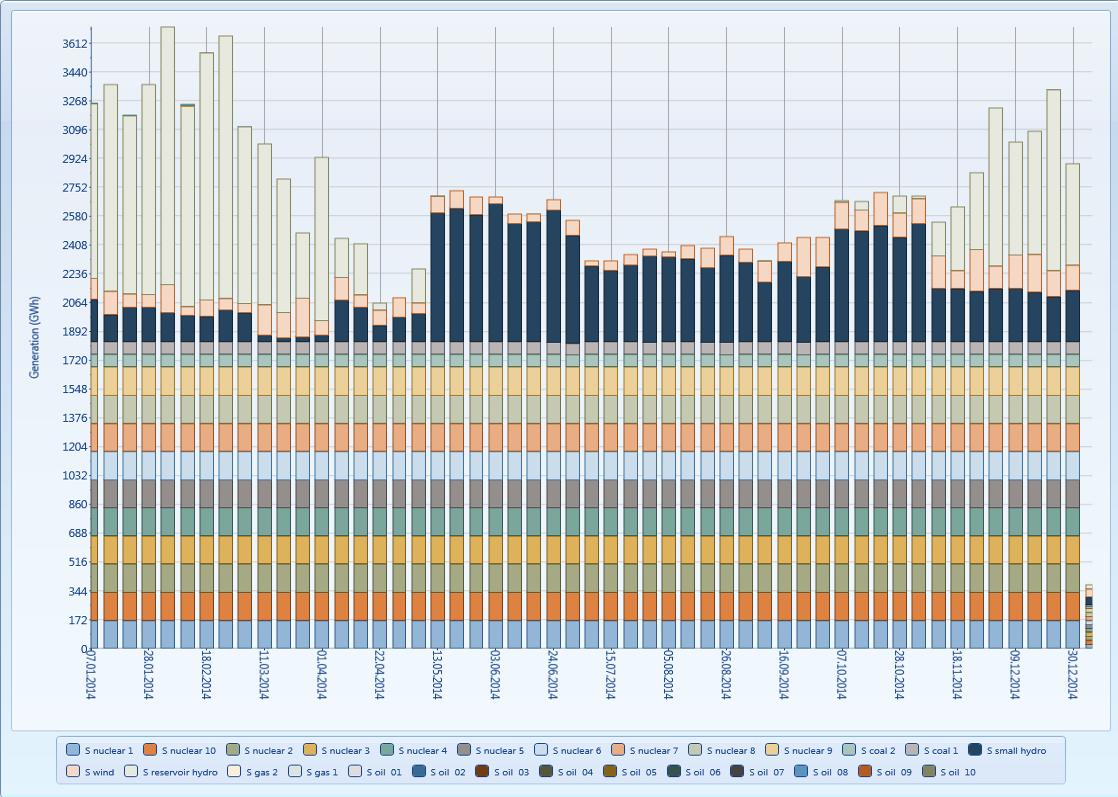
\includegraphics[width=14cm,keepaspectratio=true]{figures/MTgenerationS}
\caption{Optimal generation dispatch for Sweden 2014 with normal inflow}
\label{fig:MTgenerationSnormal}
\end{center}
\end{figure}
\begin{figure}[htbp]
\begin{center}
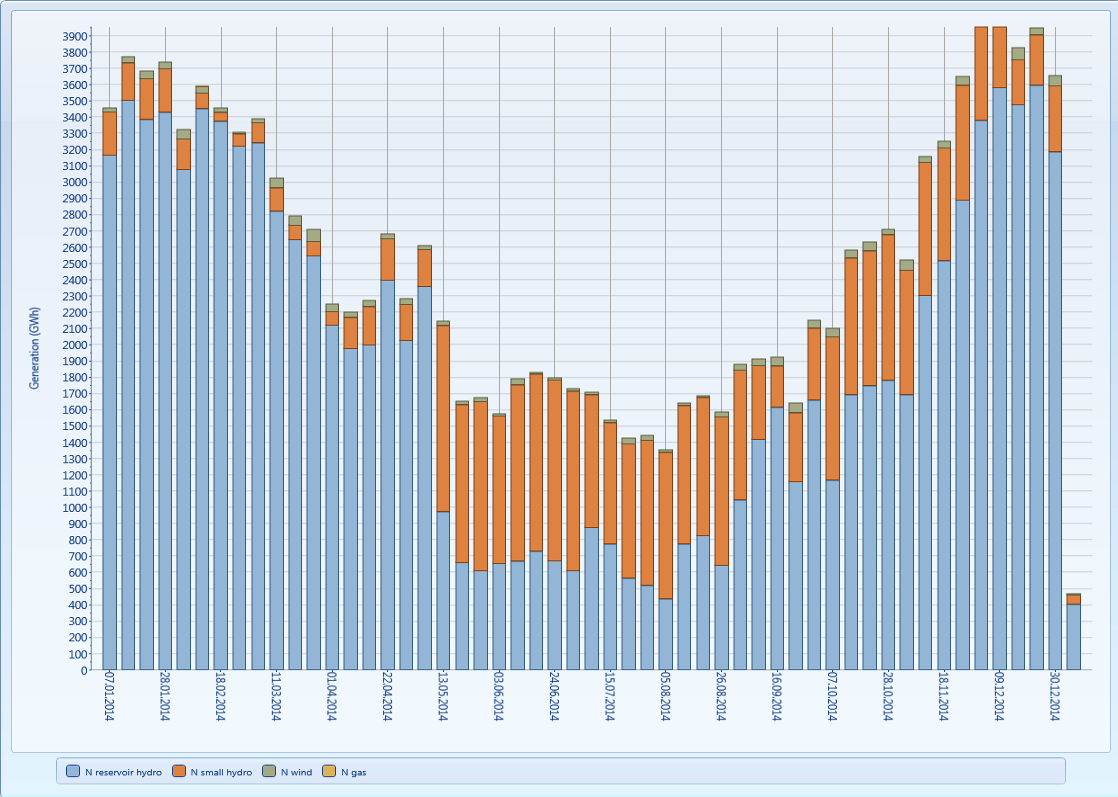
\includegraphics[width=14cm,keepaspectratio=true]{figures/MTgenerationN}
\caption{Optimal generation dispatch for Norway 2014 with normal inflow}
\label{fig:MTgenerationNnormal}
\end{center}
\end{figure}
\paragraph{transmission\\}
The transmission between the three countries Norway, Sweden and Germany is shown in figure \ref{fig:MTnodetransmission}. It is done not considering the flow direction, but the amount of power.
\begin{figure}[htbp]
\begin{center}
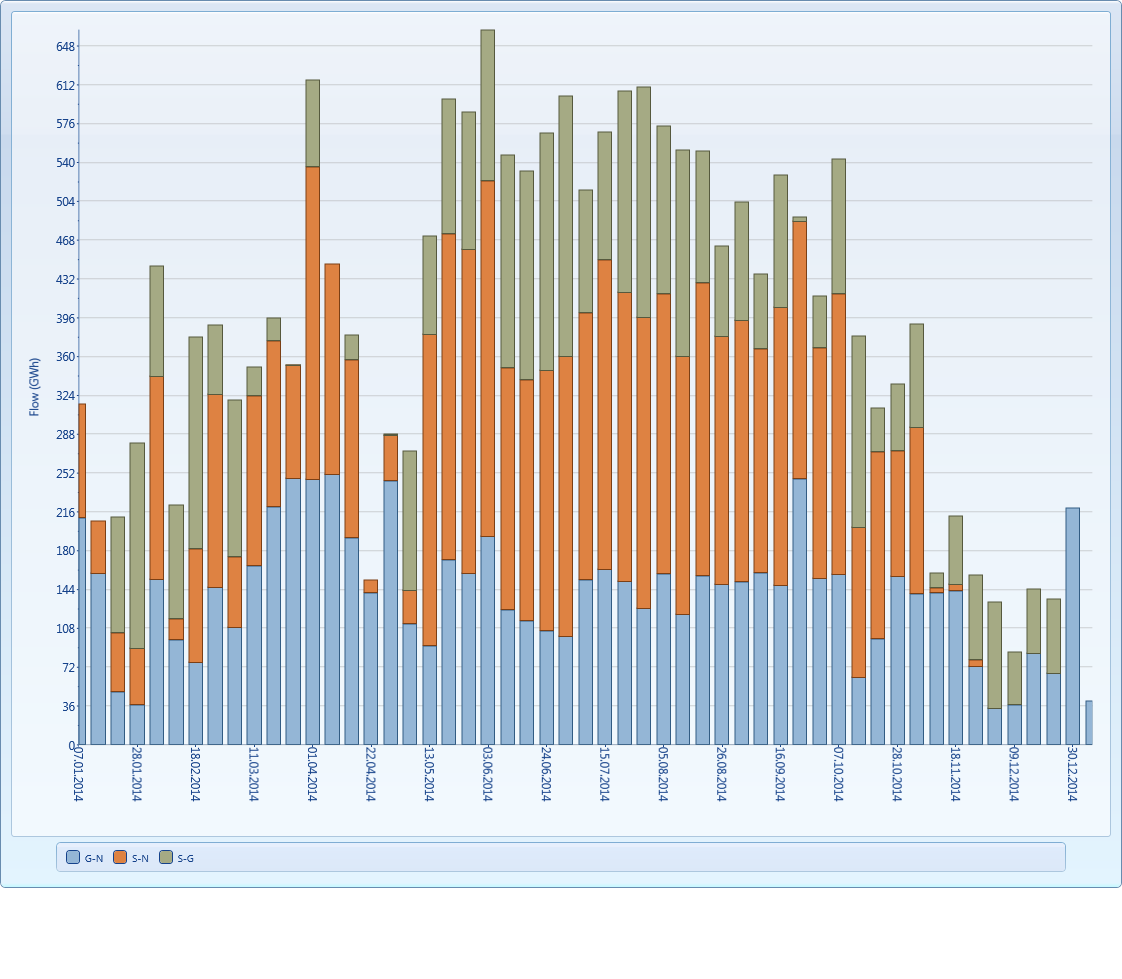
\includegraphics[width=14cm,keepaspectratio=true]{figures/MTnodetransmission}
\caption{Transmission between N/W/S with normal inflow}
\label{fig:MTnodetransmissionnormal}
\end{center}
\end{figure}
\paragraph{emission\\}
The total emissions for all countries together can be seen in figure \ref{fig:MTemissionsnormal}. The emissions can be interpreted in following way:
\begin{itemize}
\item Norway: Due to the fact that most power installed is done with renewables (hydro power, wind power) and only some small amount of gas power, there are hardly and $CO_2$-emissions in Norway.
\item Sweden: Some renewable energy and a large amount of nuclear power lead to small $CO_2$-emissions. 
\item Germany: The biggest amount of the produced emissions are emitted from german power plants. 
\end{itemize}
\paragraph{price\\}
Energy prices for the different weaks of 2014 for the analyzed countries are shown in figure \ref{fig:MTpricesnormal}.
\begin{figure}[htbp]
\begin{center}
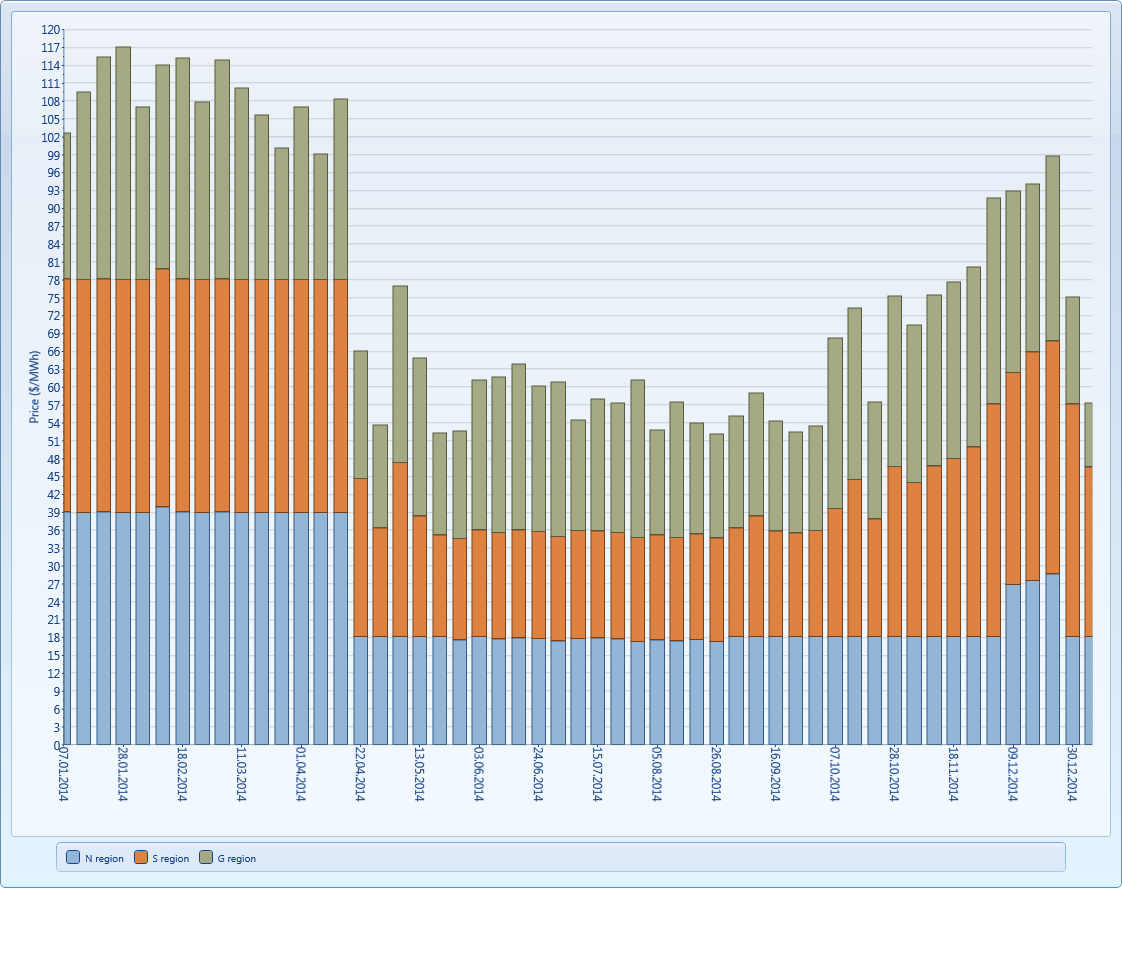
\includegraphics[width=14cm,keepaspectratio=true]{figures/MTprices}
\caption{Calculcated prices with normal inflow}
\label{fig:MTpricesnormal}
\end{center}
\end{figure}
\subsubsection{high inflow scenario}
\subsubsection{low inflow scenario}
\subsection{Expansion planning}
\newpage
\section{Conclusion}


\end{document}
